\section{The global impact of microbial pathogens} \label{sec:global_impact}

The Global Burden of Disease (GBD) 2019 study reported that microbial pathogens are responsible for more than 400 million years of life lost annually across the globe, a higher burden than either cancer or cardiovascular disease \citep{vos_global_2020}. In particular, lower respiratory infections, diarrhoeal diseases, HIV/AIDS and tuberculosis were amongst the five leading causes of global total years of life lost. More recently, the COVID-19 pandemic, declared as such by the World Health Organization (WHO) on 11 March 2020 after the emergence and global spread of the severe acute respiratory syndrome coronavirus 2 (SARS-CoV-2), and as of January 2022 has caused more than 5.63 million deaths worldwide \citep{ritchie_coronavirus_2020}, making it one of the deadliest pandemics in history. Coronavirus has been responsible for three of the eighteen major pandemics registered throughout modern history \citep{piret_pandemics_2021}, all occurring after the year 2000. \textit{Yersinia pestis}, responsible for three pandemics of plague, \textit{Vibrio cholerae}, with seven cholera pandemics, and Influenza A virus, the causative agent of five flu pandemics, are responsible for the remaining ones, with Influenza being the only other pathogen with a pandemic registered after 2000. Recent decades have also witnessed the emergence of additional virulent pathogens, including the Ebola virus, West Nile virus, Dengue virus and Zika virus, particularly in lower-income countries.

In addition to the emergence of virulent pathogens, the rise of antimicrobial resistance (AMR) poses a major threat to human health around the world. In 2019 there were an estimated 4·95 million deaths associated with bacterial AMR \citep{murray_global_2022}. In 2017, the WHO released The Global Priority Pathogens (GPP) list \citep{world_health_organization_prioritization_2017} to guide discovery, research and development of new antibiotics for drug-resistant bacterial infections (see Figure ~\ref{fig:figure1}). Besides tuberculosis, the global priority due to being the most common and lethal airborne AMR disease worldwide today, responsible for 250 000 deaths each year, it includes 12 groups of pathogens in three priority categories. 

\begin{figure*}[h!]
\centering
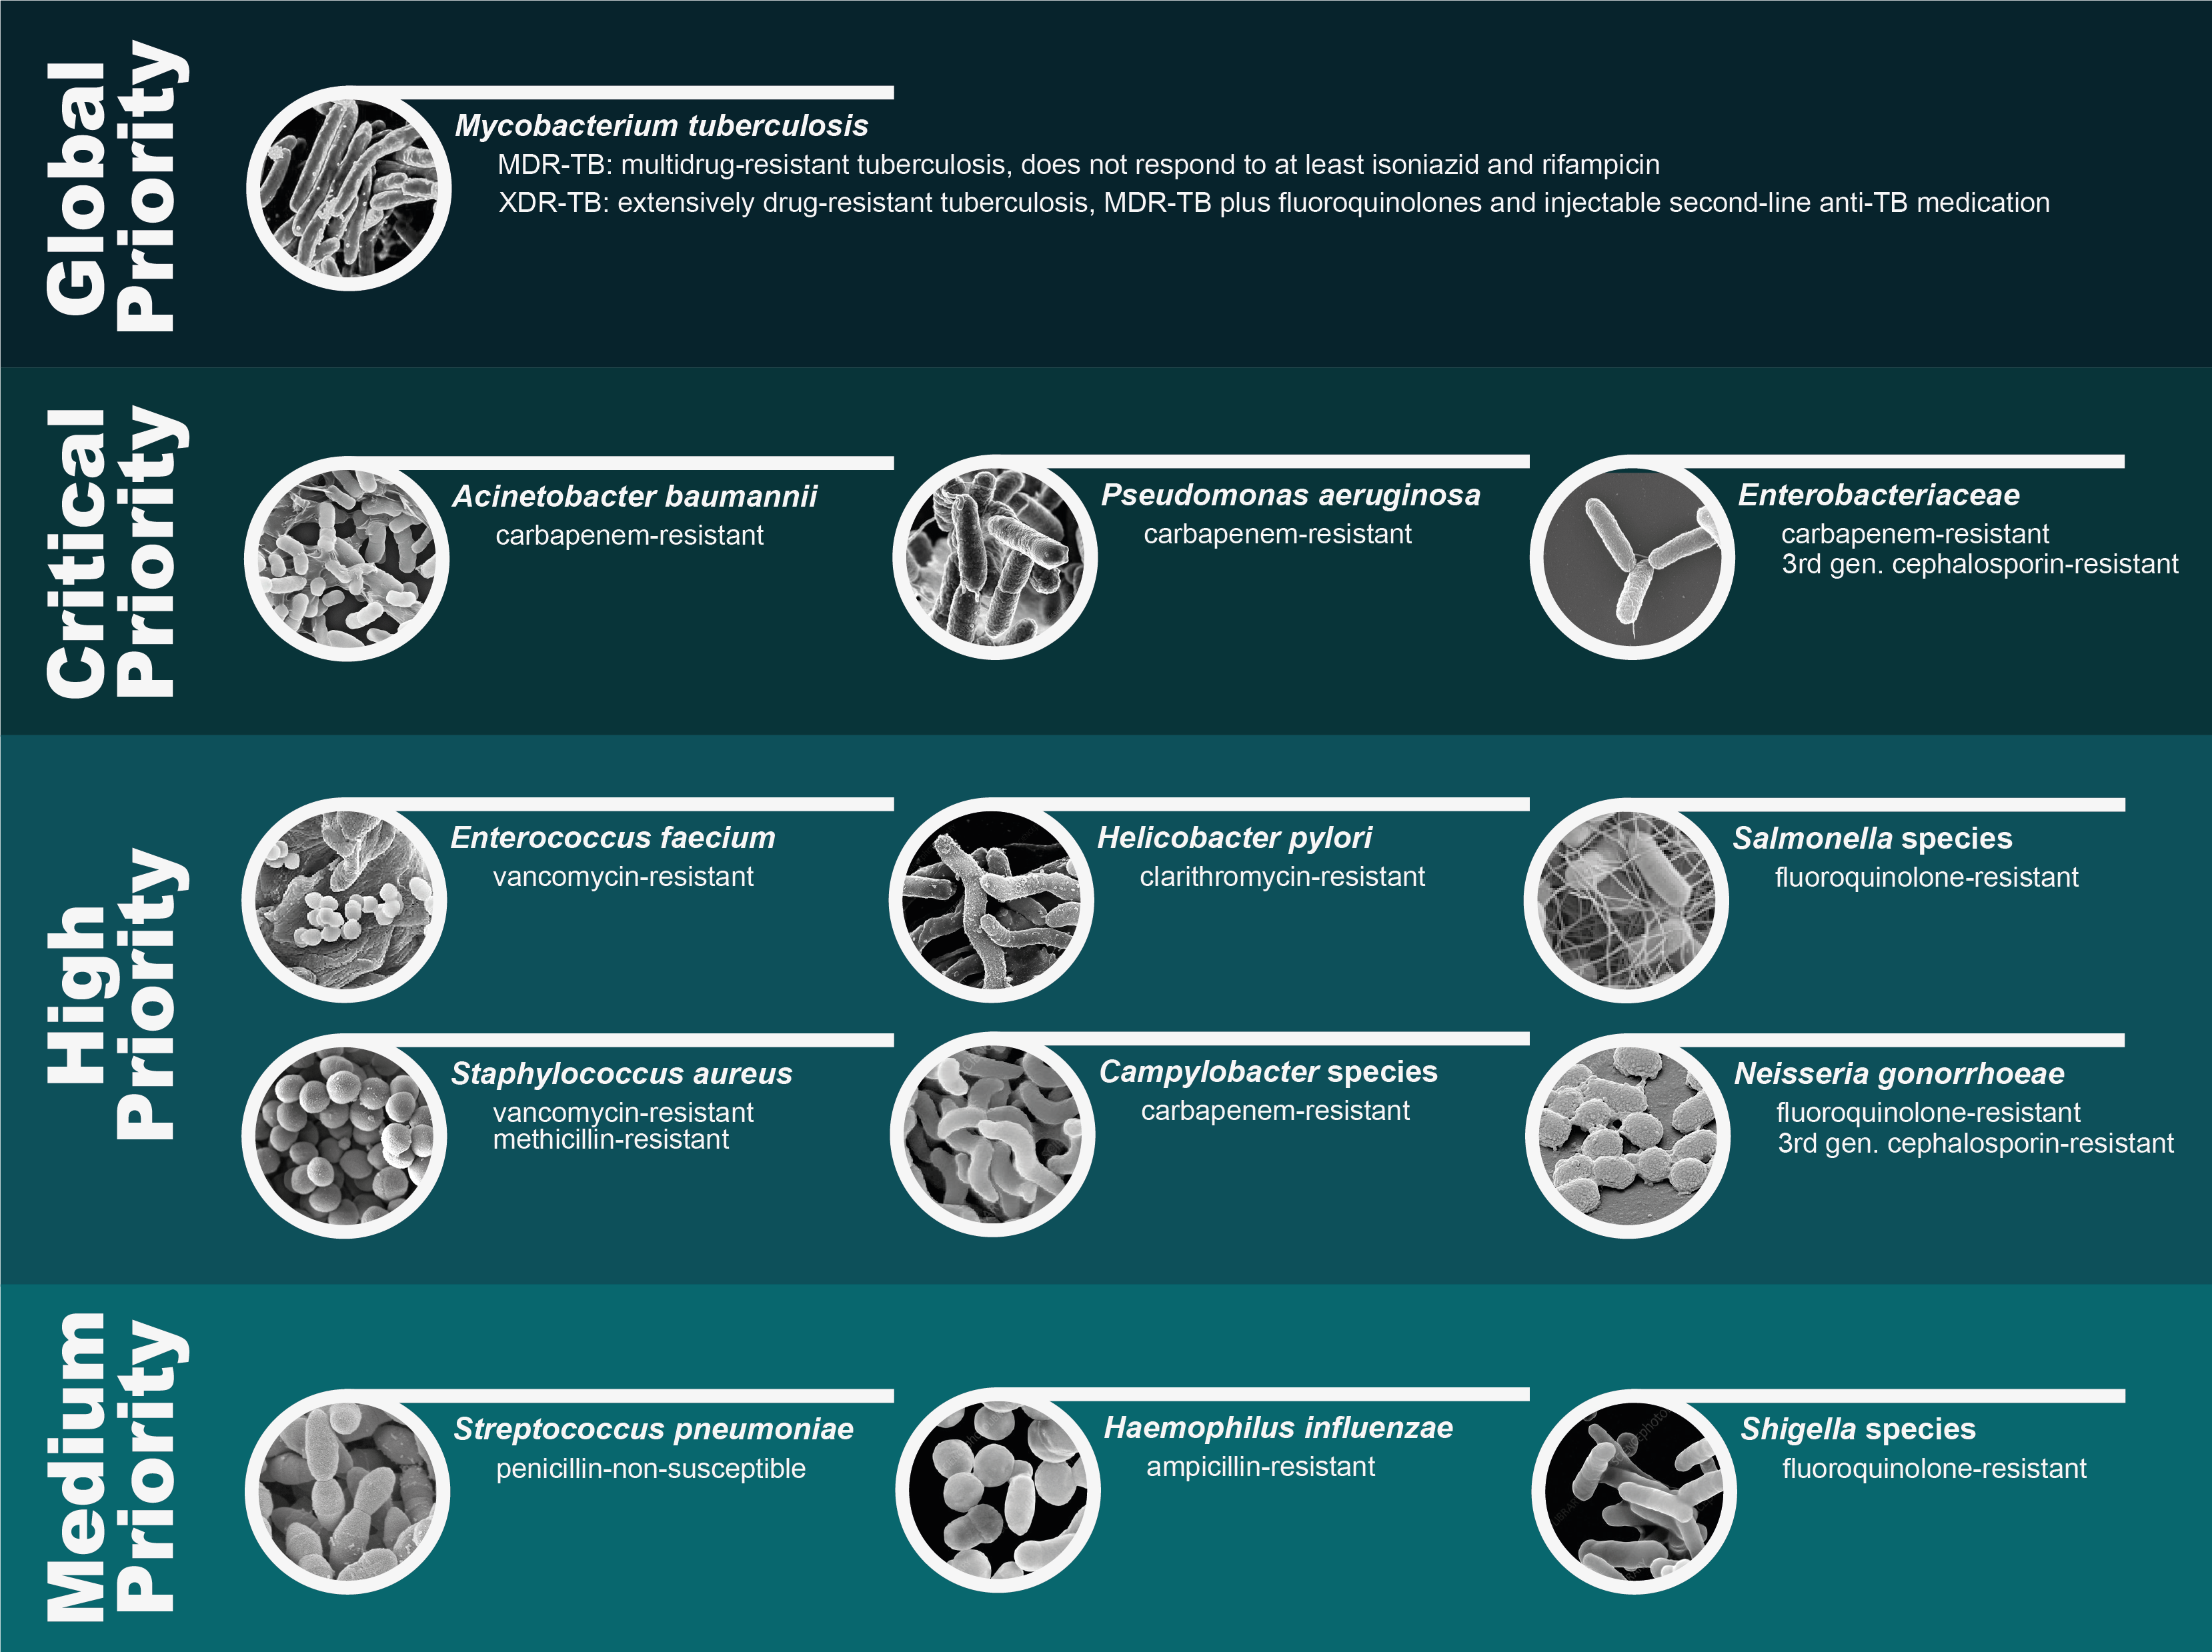
\includegraphics[width=\textwidth]{figures/introduction/Figure 1.png}
\caption{\textbf{World Health Organisation Global Priority Pathogens list.} This catalogue includes, besides \textit{Mycobacterium tuberculosis} considered the number one global priority, a list of twelve microorganisms grouped under three priority tiers according to their antimicrobial resistance: critical (\textit{Acinetobacter baumannii}, \textit{Pseudomonas aeruginosa} and \textit{Enterobacteriaceae}), high (\textit{Enterococcus faecium}, \textit{Helicobacter pylori}, \textit{Salmonella} species, \textit{Staphylococcus aureus}, \textit{Campylobacter} species and \textit{Neisseria gonorrhoeae}), and medium (\textit{Streptococcus pneumoniae}, \textit{Haemophilus influenzae} and \textit{Shigella} species). The major objective was to encourage the prioritisation of funding and incentives, align research and development priorities of public health relevance, and garner global coordination in the fight against antimicrobial resistant bacteria. Adapted from \cite{world_health_organization_prioritization_2017}.}
\label{fig:figure1}
\end{figure*}

Clinical microbiology is a discipline focused on rapidly characterising pathogen samples to direct the management of individual infected patients (diagnostic microbiology) and monitor the epidemiology of infectious disease (public health microbiology), including the detection of outbreaks and infection prevention. According to WHO's Global Expenditure on Health report from 2000 to 2019, of the 51 countries that reported health spending by disease and condition, an average of 37\% of health spending went to infectious and parasitic diseases, corresponding to the largest share of health spending \citep{world_health_organization_global_2021}. About 21\% of total health spending went to three major infectious diseases — HIV/AIDS (9\%), tuberculosis (1\%) and malaria (11\%) — and 16\% went to other infectious and parasitic diseases. On average, 70\% of external aid for health went to infectious and parasitic diseases in the 51 low and middle-income countries. Of the \$54.8 billion estimated disbursed for health in 2020, \$13.7 billion (25\%) was targeted toward the COVID-19 health response \citep{micah_tracking_2021}.

\subsection{Current standards for diagnostic in clinical microbiology} \label{ssec:current_standards}

The past few decades have seen a major revolution in the operation of microbial laboratories, driven by the development of molecular technologies and ways to make these accessible, namely amplification-based polymerase chain reaction (PCR), matrix-assisted laser desorption/ionisation - time of flight (MALDI-TOF) and DNA-microarray-based hybridisation technology. These are used in conjunction with traditional techniques such as microscopy, culture and serology, not fully replacing them. Application of these methods differs by suspected infection type: bacterial, viral, fungal or parasitic.

\subsubsection{Bacterial infections} \label{sssec:bacterial}

For patients with bacterial infections, the crucial steps are (1) to grow an isolate from a specimen, (2) identify its species, and (3) determine its pathogenic potential and test its susceptibility to antimicrobial drugs  \citep{didelot_transforming_2012}. Together this information facilitates the specific and rational treatment of patients. For public health purposes, knowledge also needs to be gained about (4) the relatedness of the pathogen to other strains of the same species to investigate transmission routes and enable the recognition of outbreaks \citep{foxman_choosing_2005}. 

The current gold standard for bacterial pathogen identification in diagnostic microbiology laboratories involves the isolation of the pathogen through culture followed by biochemical testing, a multi-step process that can take days to weeks before obtaining results, depending on the fastidiousness of the organism and if it can be cultured \citep{muhamad_rizal_advantages_2020, giuliano_guide_2019, muhamad_rizal_advantages_2020}. Although culture allows the identification of a wide variety of organisms, some pathogens can escape routine investigation due to strict metabolic necessities for growth or the requirement for specific biochemical tests needed for their identification. Additionally, results will be obscured if a mixed culture is obtained, particularly if the cultures are obtained from sites with a microbiota, such as the gut and the skin, increasing the risk of contamination from normal flora, leading to false results \citep{giuliano_guide_2019}. After successful growth in culture, Gram staining and MALDI-TOF mass spectrometry are often used for identification with good accuracy as long as the pathogen is presented in the the coexisting database \citep{patel_maldi-tof_2015}. An alternate rapid identification method is PCR where nucleic acid fragments are detected through specific probes, being highly sensitive and specific, to the point where PCR may detect bacteria that are not viable after a patient has been treated for an infection \citep{scerbo_beyond_2016}. It's limited to the probes used, with multiplex PCR, an extension of PCR by using multiple primers, tried to address this issue by allowing for the identification of multiple bacteria and other important information such as the detection of antibiotic resistance genes or virulence genes \citep{giuliano_guide_2019}

Following identification, antibiotic-susceptibility testing is essential for guiding clinicians in selecting an appropriate treatment. Conventional detection methods of bacterial resistance, such as disc diffusion, antimicrobial gradient strip and broth microdilution, are widely used but results cannot be obtained earlier than 48 hours after receiving a sample, which may lead to prolonged use or overuse of broad-spectrum antibiotics \citep{benkova_antimicrobial_2020}. Similarly to bacterial identification, MALDI-TOF and PCR have been increasingly adopted as solutions with lower turnaround times, although no phenotypic information is retrieved, nor information on the minimum inhibitory concentration (MIC) for a given antibiotic.   

Choosing an appropriate bacterial typing technique for epidemiological studies depends on the resources available and the minimum intended resolution, ranging from DNA fingerprinting to multilocus sequence typing, Pulsed-field gel electrophoresis and Sequence-based typing \citep{allerberger_molecular_2012,foxman_choosing_2005}. DNA macrorestriction analysis by pulsed-field gel electrophoresis (PFGE), which revolutionised precise separation of DNA fragments, became the most widely implemented DNA fingerprinting technique \citep{allerberger_molecular_2012}, becoming the golden standard for bacterial typing \citep{neoh_pulsed-field_2019}.

In the early 2000s, Multilocus sequence typing (MLST) was proposed as a portable, universal, and definitive method for characterising bacteria \citep{maiden_multilocus_2006}. Instead of enzyme restriction of bacteria DNA, separation of the restricted DNA bands using a pulsed-field electrophoresis chamber, followed by clonal assignment of bacteria based on PFGE banding patterns, MLST relies on the amplification through PCR sequences of internal fragments of housekeeping genes (usually 5 to 7), approximately 450-500 basepairs (bp) in size, followed by its the sequence, usually my Sanger methods. For each house-keeping gene, the different sequences present within a bacterial species are assigned as distinct alleles and, for each isolate, the alleles at each of the (usually) seven loci define the allelic profile or sequence type \citep{larsen_multilocus_2012}. As with PFGE, different schemes, defining what house-keeping gene fragments are used, are available depending on the species. Unlike PFGE, the provision of freely accessible, curated databases of MLST nucleotide sequence data enables the direct comparison of bacterial isolates, providing the basis of a common language for bacterial typing \citep{maiden_multilocus_2006}. So far, MLST schemes for 115 bacterial organisms have been published and made freely available (\url{https://pubmlst.org/organisms}, \cite{jolley_open-access_2018}) 

Depending on the organism identified, further and/or particular typing schemes can be applied. For \textit{S. pneumoniae}, one of the pathogens listed in the WHO's GPP list, the typing of the polysaccharide capsule, usually through Quellung reaction, is paramount for disease surveillance and pre- and post-pneumococcal vaccine evaluation as the capsule, with over 90 serotypes reported, is the dominant surface structure of the organism and plays a critical role in virulence \citep{jauneikaite_current_2015, paton_streptococcus_2019}. For the \textit{Salmonella} species, also in the GPP list, the serotype is usually determined by agglutination of the bacteria with specific antisera to identify variants of somatic (O) and flagella (H) antigens that, in various combinations, characterise more than 2600 reported serotypes \citep{diep_salmonella_2019}. 

\subsubsection{Viral infections} \label{sssec:viral}

The traditional approaches to the laboratory diagnosis of viral infections have been (1) direct detection in patient material of virions, viral antigens, or viral nucleic acids, (2) isolation of the virus in cultured cells, followed by identification of the isolate, and (3) detection and measurement of antibodies in the patient’s serum (serology) \citep{burrell_laboratory_2017}. Viral diagnostics is therefore generally organised into two primary categories, indirect and direct detection, depending on the method used. 

Indirect detection methods involve the propagation of virus particles via their introduction to a suitable host cell line (virus isolation), as viruses rely on host organisms to replicate. This is a relatively slow diagnostic method, sometimes taking weeks for the virus to propagate, usually followed by microscopy for its identification, or more commonly, through molecular methods with an agent which detects a virus-associated protein, such as an antibody \citep{cassedy_virus_2021}. 

Direct detection methods negate the need for virus propagation, detecting the virus directly from the suspect source through nucleic acid and immunological methods. PCR and reverse transcription-PCR are widely applied methods for the detection of both DNA and RNA viruses, respectively, driven by increased awareness of the clinical value of, and demand for, prompt information about viral loads, viral sequence data, and potential antiviral resistance information \citep{cassedy_virus_2021}. Syndromic testing, utilising multiplex PCR to simultaneously amplify the nucleic acid of multiple targets in a single reaction, is now fully integrated into the standard testing practices of many clinical laboratories \citep{dien_bard_panels_2020}. Limitations of these assays include no detection of off-target pathogens, a lack of full susceptibility information, cost, and false-positive results.

Real-time quantitative PCR (qPCR) remains the front line tool in aetiological diagnosis, measuring the production of the target amplicon throughout the reaction and providing quantitative results with high specificity and sensibility, albeit with a significant cost due to sophisticated apparatus despite high-throughput systems being widely established \citep{cassedy_virus_2021}. Immunoassays employ singular-epitope specificity antibodies as the primary means to detect viruses within a sample and provide a much more cost-efficient alternative to nucleic acid detection \citep{cassedy_virus_2021}. One major application is seroprevalence assays, an essential technique for identifying patients who have been exposed to a virus (historical exposure), detecting asymptomatic infection or evaluating vaccine efficacy  \citep{chan_determining_2021, bobrovitz_global_2021}. Lateral flow immunoassays (LFIA) are extensively used for detecting virus-associated protein directly from the source through labelled antibodies binding to their cognate antigens, usually read by way of a colour change at a test line. Besides being very cost-effective, LFAIs have a turnaround time of minutes and the colour change can be observed with the naked eye, therefore facilitating rapid diagnosis but its results are limited to semi-quantitative and it does not typically achieve sensitivity comparable to nucleic-acid detection \citep{estrela_lateral_2016, cassedy_virus_2021, di_nardo_ten_2021}.

\subsubsection{Fungal infections} \label{sssec:fungal}

Invasive fungal infections are a prevalent disease in pulmonary and critical care medicine, and they frequently pose diagnostic challenges, with laboratory diagnosis of fungal infections being identified as a key area in need of development of a clinical practise guideline \citep{haydour_diagnosis_2019}. Both serologic and molecular approaches are currently in use, with the first including not only immunodiffusion and complement fixation, both of which remain a cornerstone for fungal diagnostic testing, but also lateral-flow assays for fungal antigen detection. Molecular techniques for fungal identification both from culture and directly from patient specimens include nucleic acid probes, mass spectrometry-based methods, and nucleic acid amplification testing \citep{ramanan_laboratory_2017}. Classic fungal culture continues to be relevant and necessary, with most detection and identification methods requiring growth in culture, from phenotypic identification and staining techniques to nucleic acid hybridisation probes and MALDI-TOF mass spectrometry.  

Molecular methods of fungal identification directly from the suspect source are particularly attractive for fungi that fail to produce characteristic morphologic characters in a timely fashion, but molecular databases for fungi tend to lag behind bacterial databases in terms of maturity \citep{ramanan_laboratory_2017}. qPCR testing is one of the most frequently used
molecular methods in clinical microbiology, even days before the onset of positive culture result \citep{kourkoumpetis_polymerase_2012}. The ribosomal RNA (rRNA) gene cluster is frequently used as the target for fungi identification, as well as other targets to evaluate antifungal resistance, guiding therapy, which lowers patient mortality and decreases unnecessary antifungal treatment, improving treatment-associated costs and avoiding toxicity \citep{kourkoumpetis_polymerase_2012}. 

As with bacterial infections, typing through MLST is also performed for epidemiological studies, with public schemes being available for seven species: \textit{Aspergillus fumigatus}, \textit{Candida albicans}, \textit{Candida glabrata}, \textit{Candida krusei}, \textit{Candida tropicalis}, \textit{Geotrichum spp.} and \textit{Streptomyces spp} (\url{https://pubmlst.org/organisms}, \cite{jolley_open-access_2018}).

\subsubsection{Parasitic infections} \label{sssec:parasites}

Currently, the detection and diagnosis of parasite infections rely on several laboratory methods in addition to clinical symptoms, clinical history, travel history, and geographic location of the patient. serology-based assays, molecular-based assays and microscopy  \citep{ndao_diagnosis_2009}. The use of microscopy for the morphology-based diagnosis of the disease remains the reference standard in parasitology although identification and matching of the life-cycle stages, despite its low cost, is very challenging even with expert knowledge \citep{blasco-costa_molecular_2016}. LFAIs has been used successfully, overcoming many of the disadvantages of conventional microscopy by providing simple, quick, cost-effective, sensitive and accurate identification of parasites, particularly in low-income countries, but are available for a relatively low number of organisms, low sensitivity and reports of cross-reactivity \citep{momcilovic_rapid_2019, robert-gangneux_epidemiology_2012, rajput_false_2018}. 

As observed in the diagnosis of bacterial, viral and fungal infections, molecular methods by nucleic acid amplification through qPCR has been increasingly adopted, particularly through the commercialisation of multiplex with high sensitivity and accuracy \citep{momcilovic_rapid_2019, wong_molecular_2014}. The key limitation of molecular detection is the technological expertise and expense which are usually lacking in the field setting at highly endemic areas.

Currently, public MLST schemes for for epidemiological studies of parasitic infections are available for six organisms: \textit{Blastocystis spp.},\textit{ Clonorchis sinensis}, \textit{Kudoa septempunctata}, \textit{Saprolegnia parasitica}, \textit{Treponema pallidum subsp. pallidum} and \textit{Tricohomas vaginalis} (\url{https://pubmlst.org/organisms}, \cite{jolley_open-access_2018}).

\subsection{Surveillance and infection prevention in public health} \label{ssec:survaillance}

Infectious disease surveillance is critical for improving population health, generating information that drives action not only in the management of infected patients but also in the prevention of new ones by identifying emerging health conditions that may have a significant impact by (1) describing the current burden and epidemiology of the disease, (2) to monitoring trends, and (3) identifying outbreaks and new pathogens \citep{groseclose_public_2017, murray_infectious_2017}. Public health surveillance systems (PHSS) are composed of the ongoing systematic collection, analysis, and interpretation of data, and its integration with the timely dissemination of results to those who can undertake effective prevention and control activities \citep{teutsch_considerations_2010}. 

Traditional PHSS can have different approaches based on the epidemiology and clinical presentation of the disease and the goals of surveillance. In passive surveillance systems, medical professionals in the community and at health facilities report cases to the public health agency, which conducts data management and analysis once the data are received and communicate with the responsible entities. Globally, the WHO as described in the International Health Regulations what is notifiable by every country to WHO, such as Severe acute respiratory syndrome (SARS) and Viral haemorrhagic fevers
(Ebola, Lassa, Marburg), as well as guiding what public health measures should be implemented \citep{world_health_organization_international_2005}. Active surveillance aims to detect every case, not relying on a reporting structure, and can have many approaches from sentinel sites or network of sites that capture cases of a given condition, such as respiratory tract infections, within a catchment population \citep{murray_infectious_2017, melo-cristino_estudo_2006}. The application of environmental surveillance methods, performed prospectively to detect pathogens prior to the recording of clinical cases or to monitor their abundance in the environment to assess the potential risk of disease, has been proven as a viable alternative, particularly in wastewater \citep{andrews_environmental_2020, mcweeney_demonstration_1894, baker_combined_2011, larsen_tracking_2020}.  

"One Health" is a collaborative and multi-disciplinary approach to designing and implementing programmes, policies, legislation and research in which multiple sectors communicate and work together to achieve better public health outcomes \citep{mackenzie_one_2019}. It recognises that people’s health is closely connected to animals’ health and shared environment, focusing on zoonotic and vector-borne diseases, antimicrobial resistance, food safety, food security and environmental contamination \citep{rugarabamu_one-health_2021}.


\section{A genomic approach to clinical microbiology} \label{sec:genomics_approach}

Since the publication of the first complete microbial genome a quarter of a century ago, that of the bacterium \textit{Haemophilus influenzae} \citep{hood_dna_1996}, genomics has transformed the field of microbiology, and in particular its clinical application. The paper describing the DNA-sequencing method with chain-terminating inhibitors used in the sequencing of the first microbial genome \citep{sanger_dna_1977}, which earned the late Frederick Sanger his share of the 1980 Nobel Prize in Chemistry alongside Walter Gilbert, was, in 2014, the top fourth in the number of citations with 60335, highlighting its impact in the field of biological sciences, and by extension medicine \citep{van_noorden_top_2014}. Currently, this number has increased to 84546 according to PubMed Central\textsuperscript{\small\textregistered} (PMC) (\url{https://pubmed.ncbi.nlm.nih.gov/, https://www.ncbi.nlm.nih.gov/pmc/articles/PMC431765/}). Since its emergence, reductions in cost, technical advances in sequencing technologies and new computational developments have made genomic sequencing one of the most influential tools in biomedical research, yielding unprecedented insights into microbial evolution and diversity, and the complexity of the genetic variation in both commensal and pathogenic microbes. 

The emerging application of genomic technologies in the clinic to combat infectious diseases is transforming clinical diagnostics and the detection and surveillance of outbreaks. 

\subsection{Twenty five years of microbial genome sequencing} \label{ssec:sequencing}

Since thes discovery of the structure of DNA \citep{watson_molecular_1953}, great strides have been made in understanding the complexity and diversity of genomes in health and disease. The ability to determine the sequence in a DNA molecule  
The development and commercialisation of high-throughput, massively parallel sequencing, has democratised sequencing by offering individual laboratories, either in research or in health, access to the technology.

\subsubsection{The first-generation of DNA sequencing} \label{ssec:1st_gen_seq}

In the late 1980s, automated Sanger sequencing machines could sequence approximately 1,000 bases per day, having been applied in the 1990s to large bacterial genomes and the first unicellular and multicellular eukaryotic genomes, including the completion of a high-quality, reference sequence of the human genome under the Human Genome Project (HGP) \citep{koch_sequencing_2021, collins_human_1995}. The first genomes of the pathogenic \textit{Mycobacterium tuberculosis} \citep{cole_deciphering_1998}, \textit{Yersinia pestis} \citep{parkhill_genome_2001}, \textit{Escherichia coli} K-12 \citep{blattner_complete_1997} were sequenced using this technology, requiring years of effort and significant budgets but providing insights into the genomic complexity of these organisms. Some of the complete genome sequences produced during this era are still used today as high-quality references. 

Simplistically, in Sanger sequencing, also known as “first-generation” DNA sequencing, a DNA polymerase is used to synthesize numerous copies of the sequence of interest using dideoxynucleotide triphosphates (ddNTPs) spiked into the reaction. At each nucleotide incorporation event, there is a chance that a ddNTP will be added and the growing DNA chain will be terminated, resulting in a collection of DNA molecules of varying lengths \citep{sanger_dna_1977, hagemann_overview_2015}. Modern Sanger sequencing uses fluorescently labelled ddNTPs that allow the amplification step to be performed in a single reaction, resulting in a mixture of single-stranded DNA fragments of various lengths, each tagged at one end with a fluorophore indicating the identity of the 3' nucleotide that, after separation through capillary electrophoresis, the resulting electropherogram with four-colour fluorescence intensity can be interpreted by a base-calling software and producing 600–1000 bases of accurate sequence (reads) \citep{hagemann_overview_2015}. 

The Sanger sequencing technology remains very useful for applications where high-throughput is not required due to its cost-effectiveness, relatively low sample load and accuracy of sequencing even in repetitive genomic regions, although input DNA must consist of a relatively pure population of sequences \citep{slatko_overview_2018}. One of the most common uses is thus individual sequencing reactions using a specific DNA primer on a specific template, such as MLST of bacterial genomes. 

\subsubsection{The second-generation of DNA sequencing} \label{ssec:2nd_gen_seq}

The release of the first truly high-throughput sequencing platform in the mid-2000s heralded a 50,000-fold drop in the cost of DNA sequencing in comparison with the first-generation technologies and led to the denomination of next-generation sequencing (NGS) \citep{goodwin_coming_2016}. This trend has continued throughout the next two decades of continued development and improvement, allied to the emergence of benchtop sequencing platforms with a high-throughput of sequencing data and turnaround times of days, making it a standard in any microbiology and public health laboratories \citep{loman_twenty_2015}. second-generation sequencing methods can be grouped into two major categories: (1) sequencing by hybridisation and (2) sequencing by synthesis. 

\paragraph{Sequencing by hybridisation} \label{sssec:2nd_gen_seq_hybrid} \mbox{}\\

Sequencing by hybridisation, also known as sequencing by ligation, originally developed in the 1980s, relies on the binding of one strand of DNA to its complementary strand (hybridisation). By repeated hybridisation and washing cycles, it was possible to build larger contiguous sequence information, based upon overlapping information from the probe hybridisation spot, being sensitive to even single-base mismatches when the hybrid region is short or if specialised mismatch detection proteins are present \citep{slatko_overview_2018, detter_nucleic_2014}. Although widely implemented via DNA chips or microarrays, has largely been displaced by other methods, including sequencing by synthesis \citep{goodwin_coming_2016}. 

\paragraph{Sequencing by synthesis} \label{sssec:2nd_gen_seq_synth} \mbox{}\\

Sequencing by synthesis methods are a further development of Sanger sequencing, without the ddNTPs terminators, in combination with repeated cycles, run in parallel, of synthesis, imaging, and methods to incorporate additional nucleotides in the growing chain. All second-generation sequencing by synthesis approaches relies on a ‘library’ preparation using native or amplified DNA usually obtained through (1) DNA extraction, (2) DNA fragmentation and fragment size selection, and (3) ligation of adapters and optional barcodes to the ends of each fragment. This is generally followed by a step of DNA amplification. The resulting library is loaded on a flow cell and sequenced in massive parallel sequencing reactions \citep{giani_long_2020}
Besides having much shorter read lengths than first-generation methods, with reads ranging from 45 to 300 bases, and an intrinsically higher error rate, the massively parallel sequencing of millions to billions of short DNA sequence reads allows for the obtainment of millions of accurate sequences based upon the identification of a consensus (agreement) sequences \citep{slatko_overview_2018, goodwin_coming_2016, hagemann_overview_2015}. 

Many of the currently available sequencing by synthesis methods approaches have been described as cyclic array sequencing platforms, as they involve dispersal of target sequences across the surface of a two-dimensional array, followed by sequencing of those targets \citep{hagemann_overview_2015}. They can be further classified as either single-nucleotide addition or cyclic reversible termination or as single-nucleotide addition \citep{goodwin_coming_2016}. 

The first relies on a single signal to mark the incorporation of a dNTP into an elongating strand, avoiding the use of terminators. As a consequence, each of the four nucleotides must be added iteratively to a sequencing reaction to ensure only one deoxynucleotide triphosphate (dNTP) is responsible for the signal. The Roche 454 Life Sciences pyrosequencing device \footnote{\url{https://web.archive.org/web/20161226040638/http://454.com/}, snapshot from 26 December 2016}, was the first and most popular instrument implementing this technology, but discontinued since 2013 with support to the platform ceasing since 2016. This system distributes template-bound beads into a PicoTiterPlate along with beads containing an enzyme cocktail. As a dNTP is incorporated into a strand, an enzymatic cascade occurs, resulting in a bio-luminescence signal which is captured by a camera, which can be attributed to the incorporation of one or more identical dNTPs at a particular bead \citep{goodwin_coming_2016}. The ThermoFisher Ion Torrent system \footnote{\url{https://www.thermofisher.com/pt/en/home/brands/ion-torrent.html}}, released in 2010 and still available today, replaces the optical sensor, using instead  H+ ions that are released as each dNTP is incorporated in the enzymatic cascade, and the consequential change in pH, to detect a signal \citep{goodwin_coming_2016}. Alongside the 454 pyrosequencing system, this system has difficulty in enumerating long repeats, additionally, the throughput of the method depends on the number of wells per chip, ranging from 10 megabases to 1000 megabases of 100 base reads in length, but with a very short run time (three hours) \citep{hagemann_overview_2015, loman_performance_2012}.

The latter is defined by their use of terminator molecules that are similar to those used in the first-generation of sequencing, preventing elongation of the DNA molecule, but unlike the first methods, it's reversible. To begin the process, a DNA template is primed by a sequence that is complementary to an adapter region, which will initiate polymerase binding to this double-stranded DNA region. During each cycle, a mixture of all four individually labelled and 3'-blocked dNTPs are added. After the incorporation of a single dNTP to each elongating complementary strand, unbound dNTPs are removed and the surface is imaged to identify which dNTP was incorporated at each cluster by optical capture. The fluorophore and blocking group can then be removed and a new cycle can begin \citep{goodwin_coming_2016}. The Illumina systems, which use this technology, accounts for the largest market share for sequencing instruments compared to other platforms\footnote{\url{https://www.forbes.com/companies/illumina/?sh=774358a91aa6}}, allowing paired-end sequencing and having the highest throughput (from 25 million reads for a MiSeq instrument to  1.2 billion reads for a NextSeq instrument\footnote{\url{https://www.illumina.com/systems/sequencing-platforms.html}}), with read lengths ranging from 45 to 300 bases in length with high accuracy, albeit with long running times (4 to 55 hours), rendering this technology a good choice for many sequencing applications where large read length is not required \citep{loman_performance_2012, gupta_chapter_2014, hagemann_overview_2015}.

\subsubsection{The third-generation of DNA sequencing} \label{ssec:3rd_gen_seq}

Despite their wide adoption, second-generation methods require library preparation and an enrichment or amplification step. These steps are time-consuming, introduce biases related to preferential capture or amplification of certain regions, and produce reads with relatively small size, making transversing repetitive genomic regions impossible if they are larger than the read length \citep{hagemann_overview_2015}. Third-generation sequencing technologies, also known as long-read sequencing or single-molecule sequencing, are characterised by the generation of ultra-long-reads, albeit at a much lower throughput than the second-generation \citep{hoang_long-reads-based_2022}. They also have the potential to go beyond four-base sequencing to reveal genome-wide patterns of methylation and other chemical modifications that control the biology of bacteria or the virulence of pathogens \citep{korlach_going_2012}. Currently, commercial long-read sequencing is supported by two companies: Pacific Biosciences and Oxford Nanopore Technologies. 

The basis of Pacific Biosciences sequencers is known as single-molecule real-time sequencing (SMRT), which takes place in single-use SMRT Cells. These contain multiple immobilised polymerases which, after binding to an adaptor sequence, begins replication incorporating nucleotides with identifying fluorescent labels. The sequence of fluorescence pulses is recorded into a movie which is then converted into a nucleotide sequence. After the polymerase completes replication of one DNA strand, it continues to sequence the opposite adapter and second strand. As a result, it is possible to generate multiple passes of the same template depending on the lifetime of the polymerase \citep{hoang_long-reads-based_2022, loman_twenty_2015}. This technology has accuracy comparable with the Illumina systems but requires a higher initial investment cost, are much larger machines in comparison with the benchtop counterparts, and have much lower throughput and longer library preparation protocols \citep{hoang_long-reads-based_2022, wenger_accurate_2019}. 

Oxford Nanopore Technologies makes use of nanopores in small, portable single-molecule sequencing devices, capable of generating ultra-long sequences in real-time at a relatively low cost. Biological nanopores are embedded in solid-state membranes within disposable flow cells which, when a DNA strand passes through the pore driven by a motor protein, each nucleotide causes a change in an ionic current across the membrane, which is later base called \citep{hoang_long-reads-based_2022, loman_twenty_2015}. This process is free from fluorescence labels and amplification requirements, and after one strand is processed, the pore is available to sequence the next available strand. Sequence quality and length depend on the loaded library but are usually much lower than the alternative counterparts, and its throughput is dependent on the number and lifespan of the nanopore within the flowcell, but still much lower than the alternatives. Despite this, its portability, fast advances, and continued improvement of the flowcells make this a fast adopted technology for long-read sequencing.  

\subsection{DNA sequencing in clinical diagnosis and surveillance} \label{ssec:sequencing_diagnosis}

Whole-genome sequencing (WGS) is becoming one of the most widely used applications of microbial genome sequencing. The major advantage of WGS is to yield all the available DNA information content on isolates in a single rapid step following culture (sequencing without culture will be discussed in the \secref{ssec:metagenomics}). In principle, after obtaining a pure culture, either bacterial (see \secref{sssec:bacterial}), viral (see \secref{sssec:viral}) of fungal (see \secref{sssec:fungal}), the data from sequencing contain all the information currently used for diagnostic and typing needs, and much more, thus opening the prospect for large-scale research into pathogen genotype-phenotype associations from routinely collected data \citep{didelot_transforming_2012}.
The cost of producing massive amounts of information requires a new framework with expert handling and processing of computer-driven genomic information, as well as capable computational infrastructures, but through this technology, researchers and clinicians can obtain the most comprehensive view of genomic information and associated biological implications, transforming clinical diagnostics and the detection and surveillance of outbreaks. \citep{cirulli_uncovering_2010, noauthor_genomic_2019, goodwin_coming_2016}.

Targeted sequencing is also proving invaluable to clinical microbial and research, not only by allowing more individual samples to be sequenced within a single run, significantly reducing costs and the amount of data generated while, but also, due to the smaller target size, obtaining results with very high confidence due to the high coverage obtained \citep{goodwin_coming_2016}. This has been particularly useful in viral genomics where sections, such as the capsid, or the complete viral genome can be selectively targeted directly from the suspected sample, offering a more time-effective method to achieve the same output as traditional nucleic acid amplification methods \citep{cassedy_virus_2021}. 

\subsubsection{Sequencing in the routine laboratory workflow} \label{sssec:sequencing_routine_lab}

WGS has been used in the routine laboratory workflow when typing of pathogens by a method having the highest possible discriminatory power is required either through single nucleotide polymorphism (SNP) or core-genome/whole genome MLST analysis, for example during hospital outbreaks \citep{tagini_bacterial_2017}. Additionally, in bacterial diagnostics, WGS can be used to reveal the presence of AMR genes, or genes associated with virulence and pathogenicity, as well as to discover new genetic mechanisms for the three previously defined important clinical features of a bacterium \citep{rossen_practical_2018}. The implementation of WGS in routine diagnostics requires several adaptations in the laboratory workflow, from the ‘wet’ laboratory part (extraction, library preparation, sequencing), to the ‘dry’ bioinformatics part where genomic data is analysed and its results interpreted by specialised personnel \citep{rossen_practical_2018}. 

Currently, sequencing technologies are used in a case-by-case approach, with its adoption being much more present in a research setting than in a diagnostic one. Sequencing is mostly used after a diagnostic through the identification of the causative agent has already been performed. Although substantial advances have been made in reducing response time, most of the current systems do not yet generate enough data fast enough for a truly rapid response for it to be used in the clinical setting \citep{goodwin_coming_2016}. High-throughput DNA sequencing has found additional new applications in drug discovery and in functional genomics with, for example, SNP-based analysis to identify new drug targets \citep{loman_twenty_2015}.

Although the second-generation DNA sequencing methods have shed light on fundamental aspects of microbial ecology and function, they suffer from issues associated with short read length (see \ref{ssec:2nd_gen_seq}) and cannot reliably reconstruct long repeats because of uncertainties in mapping read, even when paired-end sequencing is used. Third-generation sequencing methods (see \ref{ssec:3rd_gen_seq}) have become increasingly used in microbiology, although their accuracy and low throughput make it challenging to implement in a clinical diagnostic setting. %CITATION NEEDED!!!

\subsubsection{Sequencing and genomic surveillance} \label{sssec:sequencing_genomic_survaillance}

Most notably, WGS has become a common tool in surveillance and infection prevention, allowing for pathogen identification and tracking, establishing transmission routes and outbreak control \citep{lo_genomics_2020}. In bacterial infections, initiatives such as Pathogenwatch\footnote{\url{https://pathogen.watch/}} offers a web-based platform for AMR analysis and phylogeny generation of \textit{Campylobacter}, \textit{Klebsiella}, \textit{Neisseria gonorrhoeae}, \textit{Staphylococcus aureus}, and \textit{Salmonella Typhi} \citep{afolayan_overcoming_2021}. The Center for Genomic Epidemiology website\footnote{\url{https://www.genomicepidemiology.org/}} offers services for phylogenetic tree building and AMR prediction. Chewie Nomenclature Server\footnote{\url{https://chewbbaca.online/}} allows users to share genome-based gene-by-gene typing schemas and to maintain a common nomenclature, simplifying the comparison of results \citep{mamede_chewie_2021}. Enterobase\footnote{\url{https://enterobase.warwick.ac.uk/}} allows for the analysis and visualisation of genomic variation within enteric bacteria \citep{zhou_enterobase_2020}. Microreact\footnote{\url{https://microreact.org/}}, from the same developers as Pathogenwatch, combines clustering, geographical and temporal data into an interactive visualisation with trees, maps, timelines and tables for a multitude of microorganisms, both bacterial and viral \citep{argimon_microreact_nodate}. Particularly for viruses, GISAID\footnote{\url{https://www.gisaid.org/}}  promotes the rapid sharing of data from all influenza viruses and the coronavirus causing COVID-19, including the genetic sequences and related clinical and epidemiological data \citep{shu_gisaid_2017}. ViPR\footnote{\url{https://www.viprbrc.org/}} provides access to sequence records, gene and protein annotations, immune epitopes, 3D structures, host factor data, and other data types for over 14 viral families, including \textit{Coronaviridae}, from which SARS-CoV-2 belongs to, and \textit{Faviviridae}, the family of Dengue and Zika virus \citep{pickett_virus_2012}. INSaFLU\footnote{\url{https://insaflu.insa.pt/}} supplies public health laboratories and influenza researchers with a web-based suite for effective and timely influenza and SARS-CoV-2 laboratory surveillance, identifying the type and subtype/lineage, detection of putative mixed infections and intra-host minor variants \citep{borges_insaflu_2018}. Nextrain\footnote{\url{https://nextstrain.org/}} provide a continually-updated view of publicly available data alongside powerful analytic and visualisation tools o aid epidemiological understanding and improve outbreak response for 10 pathogens: Influenza, SARS-CoV-2, West Nile virus, Mumps, Zika, West African Ebola, Dengue, Measles, Enterovirus D68 and Tuberculosis \citep{hadfield_nextstrain_2018}

In outbreak detection and surveillance, genetic sequencing techniques combined with epidemiological data have undoubtedly provided immeasurable insights regarding evolutionary relationships and transmission pathways in various environments \citep{beckett_pandemic_2021, lancet_genomic_2021}. In a pandemic setting, this approach, although not novel, has been revolutionary, particularly in the COVID-19 setting. 

In the 2009 swine-origin Influenza A H1N1 pandemic, the first complete genome was publicly available on the 25 of April of 2009 (GenBank accession number FJ966079), about a month after records of increased flu activity in Mexico and 10 days after the first confirmed cases in California, United States of America \citep{smith_origins_2009, novel_swine-origin_influenza_a_h1n1_virus_investigation_team_emergence_2009}. By the time the pandemic was declared, on 11 of June of 2009, \cite{smith_origins_2009} reported the origins and evolutionary genomics of the pandemic influenza A variant with a collection of 813 complete influenza genome sets, 17 of which belonging to the newly swine influenza viruses (GenBank accessions numbers GQ229259–GQ229378). The MERS pandemic, declared as such in 2015 \citep{piret_pandemics_2021}, had its first publicly available sequence on 5 of July 2015 (GenBank accession number KT006149)\citep{lu_complete_2015}, with a sequence from a camel, thought to be an intermediate host for the virus, available as early as 7 of March 2016 (GenBank accession number KU740200) \citep{kandeil_complete_2016, al-shomrani_genomic_2020}. 

The SARS-CoV-2 has brought a new meaning to genomic surveillance, with the first sequence from a COVID-19 patient being made publicly available as early as 12 January 2020 from a case of respiratory disease from the Wuhan outbreak (GenBank accession number MN908947) \citep{wu_new_2020}. At the date of the pandemic declaration by WHO, at 11 March 2020, over 400 complete SARS-CoV-2 sequences were deposited on GISAID\footnote{\url{http://web.archive.org/web/20200311053731/https://www.gisaid.org/}}, hitting over one million sequences in April 2021 \citep{maxmen_one_2021}. Currently, over 8 million complete viral sequences are available at GISAID\footnote{\url{https://www.gisaid.org/}}, being one of the most highly sequenced genomes of any organism on the planet. This richness in genomic information has been basal to identifying new variants of risk and new variants of concern with a myriad of different origins, identifying routes of transmission across borders, including the identification of "super-spreaders" events, and informing infection control measures \citep{lancet_genomic_2021, beckett_pandemic_2021, borges_sars-cov-2_2022}.  

\subsection{From genomics to metagenomics} \label{ssec:metagenomics}

Despite the increasing adoption of DNA sequencing methods in clinical microbiology, the sequencing of genetic material from a pure culture requires a priori knowledge of what to expect from a particular clinical sample or patient \citep{schuele_future_2021}. In most cases, a priori knowledge is enough to request the most appropriate test, such as multiplexed panels or specific culture media, but this is not always the case. In recent years, there has been a growing interest in using metagenomics to deliver culture-independent approaches to microbial ecology, surveillance and diagnosis \citep{loman_twenty_2015, loman_high-throughput_2012}.
Metagenomic DNA sequence allows detailed characterisation of pathogens in all kinds of samples originating from humans, animals, food and the environment, ligating the diagnostics to surveillance in a true "one health" fashion \citep{rossen__2018}. Unlike PCR or microarrays, it usually does not require primer or probe design, it can be easily multiplexed, and the specificity and selectivity of the sequencing can be adjusted computationally after acquiring the data \citep{dunne_next-generation_2012}. Whether or not it can entirely replace routine microbiology depends on several conditions and future developments, both technological and computational (see \secref{sec:bioinformatics}). 

Albeit lacking consensus in the field, metagenomics can be classified into two variants as proposed by \citep{marchesi_vocabulary_2015}: (1) metaxonomics where marker genes ubiquitous in many taxa are targeted and sequenced, and (2) the untargeted "shotgun" sequencing of all microbial genomes present in a sample. 

\subsubsection{Metataxonomics and Targeted Metagenomics}

Molecular barcoding approaches can be combined with second-generation high-throughput sequencing to achieve unprecedented depths of coverage in microbial community profiling, being defined as metataxonomics. For profiling bacterial species, the most popular approach is 16S ribosomal RNA (rRNA) gene sequencing, an ~1500 base pair gene coding for a catalytic RNA that is part of the 30S ribosomal subunit. Traditionally, the variable regions of the 16S rRNA gene (V-regions) are targeted, or ranges thereof (V1-V2, V1-V3, V3-V4, V4, V4-V5, V6-V8, and V7-V9), and are specific to bacterial genus (96\%) and for some, even species (87.5\%), \citep{srinivasan_use_2015, abellan-schneyder_primer_2021}. Moreover, dedicated 16S databases that include near full length sequences for a large number of strains and their taxonomic placements exist, such as RDP\footnote{\url{http://rdp.cme.msu.edu/}}, Greengenes\footnote{\url{https://greengenes.secondgenome.com/}}, silva\footnote{\url{https://www.arb-silva.de/}} and NCBI's 16S ribosomal RNA project\footnote{\url{https://www.ncbi.nlm.nih.gov/refseq/targetedloci/}} \citep{cole_ribosomal_2009, desantis_greengenes_2006, pruesse_silva_2007}. The sequence from an unknown strain can be compared against the sequences in these databases, after very closely related sequences are grouped into Operational Taxonomic Units (OTUs), and infer likely taxonomy, with the assumption that sequences of $>$95\% identity represent the same genus, whereas sequences of $>$97\% identity represent the same species \citep{schloss_introducing_2005}. Additionally, NCBI also provides the 23S ribosomal RNA project for Bacteria and Archaea metataxonomics. 

Because this approach is PCR-based, it suffers from the same issues described previously for conventional PCR, requiring primer design. Additionally, it must necessarily account for intragenomic variation between 16S gene copies. Microbial profiles generated using different primer pairs need independent validation of performance, and the comparison of data sets across V-regions using different databases might be misleading due to differences in nomenclature and varying precisions in classification, and specific but important taxa are not picked up by certain primer pairs (e.g., \textit{Bacteroidetes} is missed using primers 515F-944R) or due to the database used \citep{abellan-schneyder_primer_2021}. Furthermore, targeting of 16S variable regions with short-read sequencing platforms cannot achieve the taxonomic resolution afforded by sequencing the entire (~1500 bp) gene \citep{johnson_evaluation_2019}. The emergence of third generating sequencing technologies (see \secref{ssec:3rd_gen_seq}) allows for this limitation to be overcome but currently, only XXX database includes complete 16S rRNA sequences. %TODO WHAT DB

The internal transcribed spacer (ITS) region of rDNA is the most used barcode to study fungal diversity \citep{schoch_nuclear_2012}.  ITS region contains three partitions: ITS1, 5.8S and ITS2. The length of the ITS sequence is highly variable from one fungal species to another and it is strongly dependent on the primers used to target the DNA sequence. Similarly to 16S rRNA sequencing, second-generation sequencing only allows for the sequencing of one of the ITS regions (ITS1 or ITS2). Although ITS1 outperforms ITS2 in terms of richness, and taxonomic coverage, some taxa are exclusively detected only by ITS2, and vice-versa for ITS1 \citep{mbareche_comparison_2020}. This can also be remedied by third generation sequencing technologies (see \secref{ssec:3rd_gen_seq}). Similarly to 16S, dedicated ITS databases that include near full length sequences for a large number of strains and their taxonomic placements exist, such as unite\footnote{\url{https://unite.ut.ee/}}, GlobalFungi\footnote{\url{https://globalfungi.com/}} and NCBI's ITS project\footnote{\url{https://www.ncbi.nlm.nih.gov/refseq/targetedloci/}} \citep{nilsson_unite_2019, vetrovsky_globalfungi_2020}. Additionally, NCBI also provides the 28S ribosomal RNA project and 18S ribosomal RNA project for fungal metataxonomics. 

While viruses are an integral part of the microbiota, no universal viral marker genes are available to perform such taxonomic assignments. As an alternative, broad scope viral targeted sequence capture (TSC) panels offer depletion of background nucleic acids and improve the recovery of viral reads by targeting coding sequence from a multitude viral genera, such as VirCapSeq-VERT Capture Panel\footnote{\url{https://sequencing.roche.com/content/dam/rochesequence/worldwide/resources/brochure-vircapseq-vert-capture-panel-SEQ1000117.pdf}} but do not guarantee the full recovery of the viral genome, and can present biases towards certain genera \citep{schuele_assessment_2020, wylie_enhanced_2015}.

\subsubsection{Shotgun Metagenomics}

Shotgun metagenomics can offer relatively unbiased pathogen detection and characterisation, potentially able to provide genotyping, antimicrobial resistance and virulence profiling in a single methodological step. This comes with the cost of producing massive amounts of information that require expert handling and processing, as well as capable computational infrastructures. One of the biggest challenges when dealing with metagenomic data is the lack of golden standards \citep{couto_critical_2018, rossen_practical_2018}

\section{The role of bioinformatics} \label{sec:bioinformatics}


\section{Bioinformatic Analysis for Shotgun Metagenomics}

One of the biggest challenges when dealing with metagenomic data is the lack of golden standards, although major efforts are being made on the standardisation and assessment of software, both commercial and open-source \cite{} (Angers-Loustau et al., 2018; Gruening et al., 2018; Sczyrba et al., 2017: Couto et al., 2018). A plethora of open-source tools are available specifically for metagenomic data, both short and long-read data, and several combinations of these tools can be used to characterize the causative agent in a patient's infection in a fraction of the time required by the traditional methods. Alongside, there are several commercial alternatives, such as CLC Genomics Workbench (QIAGEN Bioinformatics), Taxonomer (Flygare et al., 2016) and BaseSpace (Illumina), that offer ready to use complete workflows at the cost of lack of transparency, reproducibility and control in the analysis.
Several steps that can be implemented to ensure the transparency and reproducibility of the chosen workflow. Favouring open-source tools, with clear documentation describing the methodology implemented, and stating the version of the software used and which parameters were used enables the comparison of results. This can be simplified by containerizing all the software tools with one of the many solutions available, like Docker (https://www.docker.com/) or Singularity (Kurtzer et al., 2017). The use of workflow managers, like nextflow (Tommaso et al., 2017) or the Galaxy Project (Afgan et al., 2016), will push reproducibility to the next level by taking advantage of the containerization and scalability, enabling the workflow to be executed with the same parameters in the same conditions in a multitude of different environments. The FlowCraft project (https://github.com/assemblerflow/flowcraft) leverages the combination of Nextflow and docker/singularity containers to assemble, monitor and report scientific pipelines created from the combination of pre-built components, many of them supporting metagenomic analysis.
Additional difficulties of metagenomic data are the overpowering quantities of host DNA that are often sequenced (Couto et al., 2018), making the microbial community close to undetectable, the presence of contaminants, from the bench process to the biota, and the cost associated with this methodology. They account for major caveats and must be made aware of when analysing the data.
The basic strategies for analysing metagenomic data can be simplified in the scheme in Figure 1. One of the biggest challenges when doing metagenomic analysis is differentiating between colonization and infection and to successfully discriminate between a potential pathogen and background microbiota. In the latter, when analysing samples from presumably sterile sites, like CSF and blood, it is safe to assume that all organisms found are of interest. In locations with a microbiota, the use of spiked metagenomic samples as positive control might guide the detection of the possible pathogens by comparing relative abundance between the samples. The inclusion of negative controls is essential for the correct identification of contaminants in the taxonomic results, whether originated from the sample collection, handling or sequencing process. These controls should be processed similarly to the samples and the taxonomic results should be filtered out from the final reports. 

\subsection{Quality Assessment and Quality Control}
Quality assessment and control is a basal step to any analysis, and aims to remove and/or filter low quality and low complexity reads, trim adapters, and remove host sequences from the samples’ raw data. There are many tools available but the most commonly used are FastQC (Babraham Bioinformatics) for quality control, followed by Trimmomatic (Bolger et al., 2014) or Cutadapt (Martin, 2011) to trim and/or filter adaptors, low quality and low complexity sequences. For long-read sequencing, tools like NanoPlot and NanoStats (De Coster et al., 2018), Porechop (https://github.com/rrwick/Porechop) and Filtlong (https://github.com/rrwick/Filtlong) can perform basic quality assessment and control, adapter trimming and low quality trimming respectively. 
The removal of host sequences is usually done through mapping. Bowtie2 (Langmead & Salzberg, 2012) is usually the go-tool for this process, specially as pre-build indexes of the human genome are available on-line (https://support.illumina.com/sequencing/sequencing\_software/igenome.html). The same approach can be used to remove contaminants present in the negative control by using it as reference for mapping. Alternatively for long-read, minimap 2 (Li, 2018) can map long-reads to large reference genomes, such as hg19, and the unmapped reads can be subsequently filtered with Samtools (Li et al., 2009). 

\subsection{Direct Taxonomic Assignment and Characterization}
An important information that can be retrieved directly from the quality controlled read data is the relative abundance of the detected organisms. Kraken (Wood & Salzberg, 2014) and Bracken (Lu et al., 2017), Midas (Nayfach et al., 2016), Kaiju (Menzel et al., 2016) and MetaPhlAn 2 (Truong et al., 2015) are all examples of taxonomic classifiers for short-read raw sequencing data that provide information on relative abundance. All tools provide a reference database. Kraken offers several pre-built databases constructed from complete bacterial, archaeal, and viral genomes in RefSeq (as of Oct. 18, 2017), known as MiniKraken, that range in size to accommodate limited computational resources, as well as providing the option to build the standard database given that the required computational resources are met. Midas and MetaPhlAn also provide a default pre-built database, with resolution down to strain level. Kaiju differs from the other tools by using a protein reference database but no pre-built version is available, requiring significant resources to build and index the database pre-use. 
The long-read data can be treated as single-end fastq, after proper conversion in the basecalling process. All tools mentioned accommodate classification of single-end files. 
16S classification can also be performed, for validation purposes, by extracting the reads of interest through HMMER (Wheeler & Eddy, 2013) and then perform a traditional OTU analysis with Quiime2 (https://qiime2.org/) or MapSEQ (Rodrigues et al., 2017).  
For virulence gene detection and antimicrobial resistance characterization a mapping approach, with an adequate database, is usually followed, using as reference the Virulence Factors Database (Chen et al., 2016), and ResFinder (Zankari et al., 2012) or CARD (Jia et al., 2017) for antimicrobial resistance gene detection. Besides mapping, other strategies have been applied, like Mash Screen (Ondov et al., 2016), that offer similar results in a faster way.  Similar strategies can be applied to plasmid detection by using the PlasmidFinder (Carattoli et al., 2014) or RefSeq plasmid (O’Leary et al., 2016) databases. The minimap 2 tool (Li, 2018) is a good alternative to map long-read data to any of the resistance and virulence databases mentioned. 
It is possible to genotype the bacterial population in a metagenomic sample, but only for short-read sequencing data.  MetaMLST (Zolfo et al., 2017) reconstructs the MultiLocus Sequence Typing (MLST) loci directly from the sequencing data and provides a pre-built database for the analysis.

\subsection{Metagenome Assembly}
Several limitations arise when using just the sequencing data. Although relatively fast and providing quantitative information, it’s strictly dependent on the content of the databases used. In addition it lacks context information, as linking the characterizing information to a given identified organism isn’t possible. 
Longer sequences are more informative than shorter sequencing data and can provide a more complete picture of the microbial community in a given samples. Several dedicated metagenomic assembly tools are available, such as metaSPAdes (Nurk et al., 2017)  and MegaHIT (Li et al., 2015). These tools, in comparison to single-cell data assemblers, are better at dealing with the combination of intragenomic and intergenomic repeats and uneven sequencing coverage (Olson et al., 2017). Assembler using multiple k-mers, like the ones suggested, substantially outperform single k-mer assemblers, and smaller k-mers improve the recovery of low-abundance genomes, larger k-mer lead to a better recovery of highly abundant ones (Sczyrba et al., 2017). 
For long-read data, no dedicated metagenomic assembler is not yet available, but several assembler for long-read data as available, including Canu (Koren et al., 2017) and Unicycler (Wick et al., 2017). The latter allows for hybrid assemblies to be constructed, combining short and long-read information to produce the best assembly possible. Nevertheless, the use of non dedicated assemblers for metagenomics may come with the cost of wrongly interpret variation as error, especially in samples that contained closely related species and the construction of chimeric sequences (Teeling & Glockner, 2012) as traditional assemblers follow the basic principle that the coverage in a sample is constant. 
The assembly-based approach requires the grouping of the different contigs into bins, ideally each collecting the sequences that belong to a microorganism present in the sample. The binning process can be taxonomy dependent, relying on a database to aggregate the sequences, or independent. The independent approach has the benefit of not relying on a database, but instead it uses the composition of each sequence and coverage profiles to cluster together sequences that might belong to the same organism. These algorithms don’t require prior knowledge about the genomes in a given sample, instead relying on features inherent to the sequences in the sample. Although most binning softwares can work with single metagenomic samples, most make use of differential coverage of multiple samples to improve the binning process (Sedlar et al., 2016). It allows the handling of complex ecosystems and might be crucial when analysing samples recovered from sites with a complex microbiota. 
A comparison of five taxonomic independent binning softwares and four taxonomic binning softwares (Sczyrba et al., 2017) revealed that, for taxonomic independent approaches, MaxBin 2.0 (Wu et al., 2016) had the highest completeness and purity in the bins obtained, with ~20\% better results in comparison with the second best ranked tool. For taxonomic binning, working similarly to the direct taxonomic assignment of the sequencing data, PhyloPythiaS+ (Gregor et al., 2016) obtained better results in accuracy, completeness and purity, followed by Kraken (Wood & Salzberg, 2014) that still obtained decent results with the added benefit of very high speed of analysis, ease of use and inclusion of the pre-built databases.
The last step on the assembly methodology is the evaluation of the completeness and contamination of the bins. When using a taxonomic binner, the effects of contamination are mitigated as the sequence clustering is performed based on matches with reference database. The contaminants, if present in the database, will be separated into different bins or just added to the bin of unclassified sequences. When using a taxonomic independent binning software, the composition and abundance might not be enough to discriminate between all the organisms, with the possible result of having bins with contaminating sequences of other organisms present in the sample. CheckM (Parks et al., 2015) assesses the quality of the recovered genomes, estimating completeness and contamination by evaluating ubiquitous single-copy genes. 
Another problem with metagenomic assembly is the high number of ambiguities that fail to being resolved, mostly due to the possible presence of several strains of the same species or species that are closely related. When faced with this ambiguities the assembler usually breaks the sequence, leading to fragmented reconstructions of genomes. MetaQUAST (Mikheenko et al., 2016) that besides computing several metrics to evaluate assembly quality like number of contigs, maximum contig length, etc, also uses reference-based method, either provided by the user or by identifying the appropriate reference sequences by 16S ribosomal RNA identification, to identify mis-assemblies and structural variants. VALET (https://github.com/marbl/VALET) is a de novo pipeline for detecting mis-assemblies without the need for references, relying instead on coverage and length to do the assignment, as well as providing severa visual representations of assembly quality. After the mis-assemblies have been detected, they can be visualized in Icarus (Mikheenko et al., 2016) for metaQUAST, or IGV (interactive genome viewer) for VALET. Anvi’o (Eren et al., 2015) is an analysis and visualization platform that empowers binning refinement and genome completeness and contamination evaluation with interactive interface. 
All downstream processes used in single cell genomes can be applied to each of the resulting binned genomes, that now represent a taxonomic unit recovered from the original metagenomic sample. The typical workflow usually involves antimicrobial resistance and ccvirulence detection. Similar approaches can be used as described in the Direct Taxonomic Assignment and Characterization section by using alignment methods, such as BLAST (Altschul et al., 1990) or DIAMOND (Buchfink et al., 2015), to compare against the Virulence Factors Database, and the ResFinder or CARD databases. Genotyping can be done through the mlst software (https://github.com/tseemann/mlst). The reconstructed genomes allow for the use comparative genomics against other references by using, for example, cgMLST or SNP analysis, and playing a major role in early outbreak detection. 


\subsection{Virus and Eukaryotes in Metagenomic Analysis}
One of the biggest advantages of using metagenomic methods is the detection of not only bacterial organisms, but also viral and eukaryotic pathogens. 
Besides the limitations inherent to the metagenomic process, the retrieval of viral genomes from clinical samples has added difficulties. The fragments of viral genomes are typically orders of magnitude less abundant, the viral genomes often deviate considerably from reference genomes, and the high intrapopulation viral diversity can lead to ambiguous sequence reconstruction or broken assemblies (Rose et al., 2016). Adding to this, the relatively few viral reference genomes can render classification problematic. For fungi, there’s an underrepresentation of the diversity of this group in databases as it remains understudied compared to bacterial microbiomes (Donovan et al., 2018).
Of the tools mentioned for read classification, Kraken’s MiniKraken and MetaPhlAn 2 databases is the most inclusive, including information of virus, bacteria, human and fungi. None other method of the ones described in this review provide a database as inclusive but many, such as Midas, allow the user to build custom databases although requiring very high computational power. Alternatively, the assembly based method can be implemented followed by an alignment search to a database that includes fungi and viral genomes, such as NCBI’s RefSeq (O’Leary et al., 2016) or GenBank (Benson et al., 2005). 
